\documentclass[a4paper,twoside]{article}
\usepackage{subfigure}
\usepackage{calc}
\usepackage{amssymb}
\usepackage{amstext}
\usepackage{amsmath}
\usepackage{amsthm}
\usepackage{multicol}
\usepackage{pslatex}
% added packages
\usepackage{booktabs}
\usepackage{paralist} % pour des listes en ligne
\usepackage{multirow} % pour des listes en ligne
\usepackage{varioref} % pour les références relatives
\usepackage[T1]{fontenc}
\usepackage[utf8]{inputenc}
\usepackage[english]{babel}  % gestion de la langue
\usepackage[xindy,acronym]{glossaries} % gestion des glossaire
\usepackage{natbib} % gestion de la bibliographie
\usepackage{graphicx} % gestion des images
\usepackage[super]{nth}
\usepackage{url}

\newcommand{\V}{\mathcal{V}}
\newcommand{\U}{\mathcal{U}} 

\makeglossaries
\loadglsentries{glo-csedu19}
\subfigtopskip=0pt
\subfigcapskip=0pt
\subfigbottomskip=0pt
\usepackage{SCITEPRESS} % Please add other packages that you may need BEFORE the SCITEPRESS.sty package.

\begin{document}

\title{Towards Visuals Explorations of Forums' Collective Dynamics in Learning Management Systems}

%\author{\authorname{Malik Koné\sup{1,2}, Madeth May\sup{1}, Sébastien Iksal\sup{1}, Souleyman Oumtanaga\sup{2}}\affiliation{\sup{1}LIUM, Le Mans Université, Le Mans, France}\affiliation{\sup{2}LARIT, INP-HB, Yamoussoukro, Côte d'Ivoire}\email{\{malik.kone, madeth.may, sebastien.iksal\}@univ-lemans.fr, oumtana@gmail.com}}

\keywords{Visualization, Forums, Collective Learning, Learning Analytics}
\abstract{
  Discussion and exchange among peers have been hailed as an essential part of learning since, at least, Vygotsky's socio-constructivist theory.  There, learning is presented as a subtle and dynamical collective process.  Hence, despite numerous efforts to understand how learners engage and maintain inspiring discussions, researchers continue to question how to reinforce effective collective actions.  In \glspl{lms} they propose \glspl{ldb} to learners, tutors, and managers to help them monitor various learning indicators.  But only recently have they employed  \glspl{nlp} and \gls{sna} techniques to display temporal indicators incorporating the forums' content analysis and the learners' behavioral patterns.
  In this study, we present our design efforts to model a scalable and portable indicator of collective actions.  We aim to support tutors monitor forums' activities through explorable visualizations.  We review previous researches about visuals explorations of Forums' content and online collaboration's measures and expose in progress visualizations built from three different datasets.
}

% on data overload (Borges & Baranauskas 2003, Dyckhoff, 2012)
% on importance interaction in forum as application of socioconstrutivsime Ferguson
% on mirroring feedback importance ?? kay 2005
% on visualization provoking understanding and self-reflexion (duvall 2011, klerkx 2014)

% TEL, LN,
\onecolumn \maketitle \normalsize \vfill

\section{Introduction}
% reseting glossary entries
\glsreset{lms}
\glsreset{ldb}
\glsreset{nlp}
\glsreset{sna}
% what's the problem ?
Modern online learning environments rely on forums or chat room to allow their students to exchange information about the subject, get help from peers and tutors or discuss informally.  When attendance is massive --as in currently popular \glspl{mooc}--, or if the course session spread over a long period of time, the messages in the forums rapidly become intractable.  Therefore, the mass of information is devalued and can even be a burden on the learners as they struggle to find adequate peers to support learning collectively.

Efforts have been made to help tutors analyzes the students' exchanges in forums but, as we will see in section.~\ref{section:3}, these analyzes are often limited to a small set of individual or topic specific.  Also, they often come at the end of the learning session and do not allow guidance.
% They could be improved by adding a temporal dimension and refining the semantic dimension.

Meanwhile, interactions taking place in forums are hailed as essential aspects of the socio-constructivism learning theory.  Vygotsky emphasizes the importance of discussions as they take learners at the fringe of their knowledge (the proximal development zone) helping them to push back their knowledge frontier and build some new.

Therefore, facilitating forum usage in ways that encourage discussions and collective actions should theoretically be beneficial to the learning experience of all actors.  But as far as we know, there is yet no method to come up with a generic and dynamic way to explore the social interactions taking place in \gls{lms}.  Learners often struggle to build a sense of belonging \citep{Khalil2014} and tutors have difficulties supporting effective collective actions \citep{Zheng2015}.  The learning potential brought by the popularization of \gls{lms} is hindered.
(%ref bandura)

% why should one get interested in visualization of collectiv dynamics ?

Well-designed learning dashboard could help support collective actions by enabling the exploration of the forums' interactions.  They would offer the possibility for the tutor and administrator to better understand how students and discussed topics evolve, as well as facilitate the curriculum design improvements.  \glspl{ldb} could also help learners develop reflexive competencies and increase their engagement.
% (ref Zimmer)

% What benefits would be get from improving it ? or why do we need to improve it ?

In this paper, we report our first step towards facilitating collective activities with tools supporting the tutor in their visual exploration of VUIC's forums.

% explore design guideline to build interactive visualizations showing the collective dynamics in \glspl{lms}' forums.  Our objective is to propose a method to generate these visualizations independently of the corpus and, in fine, to facilitate collective actions.

In the next section we define collective dynamics and explain why we see it differently from collaboration.  Then, in section~\ref{section:3}, we recall previous efforts made to  monitor collective actions and use \glspl{ldb} as support tools.  In section~\ref{section:4}, we present our model and propose a way to come up with an interactive visualization (or explorable) of the forum's collective dynamic.  We illustrate it, in the \ref{section:5}\sup{th}~section with our firsts visualizations built from different datasets that we will have detailed in the preceding section.  Finally, we discuss our visualizations' limitations and future developments in section~\ref{section:6}.

\section{Visualization of Collective dynamics in \glspl{lms}}
\label{section:2}

The first clarification we make is between a visualization and a \gls{ldb}.  A Learning Dashboard is a ``single display that aggregates different indicators about the learner learning process and or learning context into one or multiple visualizations'' \citep{Schwendimann2017}.  We will use the term visualization when the \gls{ldb} can be made of single visualization and keep the term \gls{ldb} when it incorporates clearly several visualizations.

Also, we will consider discussions taking place in \glspl{lms} or in other online applications if the latest is used in an educational context.  We understand that \glspl{lms} are applications designed with the intention of being teaching tools, but sometimes we may refer to Hangout as an \gls{lms} too.   If so, it is because we consider the specific Hangouts chat from G Suite for Educational which was built with the intent of being a support to teaching.

We collected 7 datasets from Coursera, Hangouts and Moodle.  The datasets are different in size and quality.  The means of collection and the dataset specificity are detail in Table~\ref{tab:datasets} and Section~\ref{section:4}.  

\subsection{Actions in forums}

\begin{figure}[b]
  \small{
    \caption{\label{fig:discussion}
      Illustration of how the strength of actors' ties (or links) varies as a function of time and topic overlap.  Thread 1 corresponds to actor--topic dynamic (\ref{eq:1a}) where $B$'s late post after $A$'s \nth{1} publication does not correlate strongly enough to create the link from $A$ to $B$. But $A$'s \nth{2} post is timely enough, although not exactly on the same topic as $B$'s message, to create the tie $B \dashrightarrow A$ drawn as a dashed arrow.  In thread 2, in addition to the tie $A \dashrightarrow B$, we have a topic overlap and time proximity between $C$ and $A$.  This makes a the strong tie $C \to A$.
    }}
  \centering
  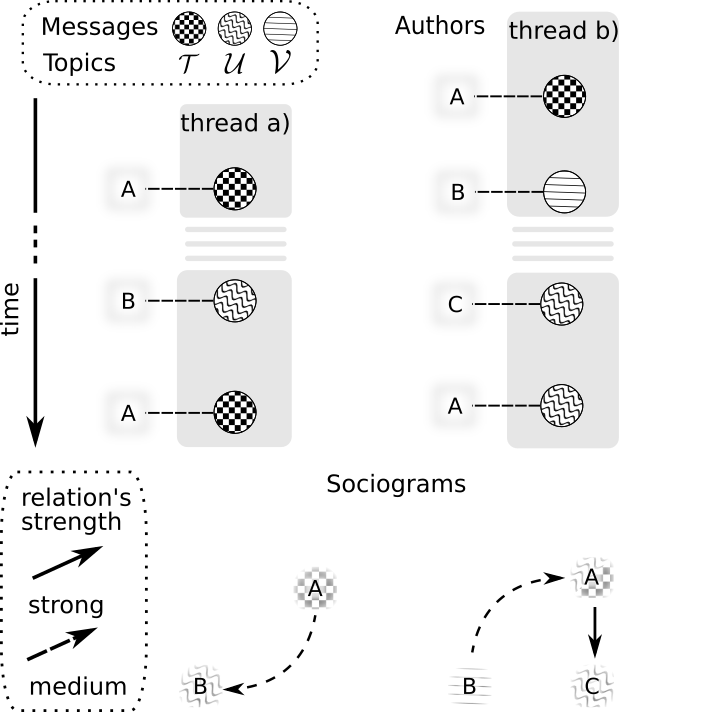
\includegraphics[width=.45\textwidth]{images/discussion.png}
\end{figure}



We make an important distinction between collaborative actions and collective actions.  \cite{Dillenbourg1999} define collaboration as a coordinated synchronous activity born from the persistent will to share a common perception of a problem originating from people with similar social roles.  It is difficult to analyze automatically collaboration if we take it as a bottom-up process with the order coming up from the actors themselves.  It implies that to coordinate, each actor has to evaluate the intentions of others and doing so, instantiate a theory of mind \citep{Gerstenberg2017}, which is very challenging to implement.  Therefore we use the term ``collective action'' instead of ``collaboration'' to emphasize that we do not make any assumption about the actors' intentions.  We focus on a set of observable actions and leave the deduction of the causal relationship to the observer.

The elementary actions we are most concerned with are those taking place in forum and chat rooms of \glspl{lms}.  They mostly are publications and message comments, but messages' up and down vote, publication times are significant and integrated in the model that we elaborate in section~\ref{section:4}.

\paragraph{Forums and Chat}

Depending on the \gls{lms}, different tools exist to facilitate discussions between peers. The main distinction is historical and separated asynchronous tools, forums, from synchronous aimed chat rooms.  Hence, forums' hierarchical structure is often more elaborated than that of chat rooms because their posts were always meant to be persistent.  On the other hand, chat rooms have better online awareness and presence indicators.

In this study, we consider that a forum is made of discussions and that each discussion is created from an initial message followed by other messages.  This sequence of messages is what we call a discussion thread.  A discussion may contain several threads if comments are allowed or if explicit references are made to previous publications.   In that case, the new thread will contain the referenced messages up to the initial one and all subsequent comments.  In chat rooms, several interrelated threads may also appear in a unique discussion when one explicitly mentions a previous message.

Despite their historical differences, today, both forum and chat room can be used for synchronous and asynchronous online discussions.  One can subscribe to a forum's discussion and receive alerts as soon as a new message is published.  In chat rooms, a history of posts is now kept and creation of several co-existing chat rooms has been facilitated.  Each chat room is them equivalent to a forum discussion. Finally, both forums and chat rooms display messages' timestamp and authors' information.
So for simplicity, we will call indifferently ``forum'' the forums described above or the chat rooms.

\subsection{Collective Dynamics}

% what do you mean by colletive dynamics
Collective dynamics are time-dependent interactions spurring for the messages co-occurrence in the forums' discussions.

\paragraph{Elementary dynamics}

\subparagraph{Actors' messages dynamics}
How do actors' messages spread over time ?  Let $(\tau_i)_{1, 2, 3}$ be three messages timestamp and $A$, $B$, $C$ three actors.  Collectively, the actors' messages could be distributed as $A_1, B_2,C_3$, meaning that $A$, $B$  and $C$ respectively posted one message at timestamp $\tau_1, \tau_2, \tau_3$.  But another dynamic could be that actor $A$ alone published the three messages, thus $A_1, A_2, A_3$,  or alternatively that $A$ published a message at $\tau_1$ and $B$ at timestamp $\tau_2$ and $\tau_3$, thus $A_1, B_2, B_3$.  Theses denotes different dynamics for the actors messages.  Visualizing them would help identifying the users posting behavior and distinguish active learners from lurkers and behavioral categories.

% ref see Medina despero, stahl 2014
% on tie strength (Granvetter 1973, Friedkin 1982)

\subparagraph{Topics' messages dynamics}
How do messages spread over time and topics ?  Or how topics are covered by messages over time ?
% Taking the previous timestamps  $(\tau_i)_{1, 2, 3}$, we could also be interested in viewing what topics were covered by messages over time.
\gls{lda} based methods are commonly used Bayesian parametric methods to approximate a message's topic or topics mixture \citep{Jelodar2017}.  To map each message to a point in topic space $\Phi$ we can also use other statistical non parametric methods such as stochastic block model \citep{Gerlach2018}.   The aim is to represent a message $M$ in the topic space which can be, for example, the set of probability distributions over $\Phi = \T\times \U \times \V$ where a point $M = (.7, .1, .2)$ denotes that the message is made of topics $\T$, $\U$ and $\V$ respectively in proportions $.7$, $.1$ and $.2$.  To simplify the next examples we suppose that each message maps to a unique topic. $M$ from topic $\T$ would be the point $(1, 0, 0)$.

A simple topic message dynamics example is  $\T_1, \T_2, \T_3$,  where all three messages are in the topic $\T$.  At the opposite we could have $\T_1, \U_2, \V_3$ where each message maps respectively to topics $\T$, $\U$ and $\V$.

This type of dynamic can show the evolution of the hot topics in the \gls{lms}, and how topic interest evolves over time.


\paragraph{Actor--topics' dynamics}
How does actors' messages cover topics over time?  Let $(A\T)_i$ be the message with timestamp $\tau_i$ posted by actor $A$ and on topic $\T$.  The two threads in Figure~\ref{fig:discussion} illustrate the following actor--topics dynamics:


\begin{subequations}
  \begin{align}
    \label{eq:1a}
    (A\T)_1, \cdots{}, (B\U)_8, (A\T)_9
  \end{align}
  \begin{align}
    \label{eq:1b}
    (A\T)_1, (B\V)_2, \cdots{},  (C\U)_8, (A\U)_9
  \end{align}
\end{subequations}

(\ref{eq:1a}) denotes that actor $A$ published two messages both on topics $\T$, but the \nth{2} came after $B$'s message on topic $\U$ that was published long after (${}_1,\cdots, {}_8$) $A$'s \nth{1} message.

In (\ref{eq:1b}), $B$ publishes a message on topic $\V$ immediately after $A$'s message on $\T$.  Then, after some time and other publications, $A$ posts a message on yet a \nth{3} topic $\U$, similar to what $C$ had just published on.

We start to make a relationship between the actors' interests and the popularity of topics.

\paragraph{Compound dynamics}
From the above observable dynamics, we can define two more dynamics: the actor--actor and topic--topic dynamics.

\subparagraph{Actor--actors' dynamics}

The actor--actors' dynamics can be taken as the evolution of the actor's social network where actors are linked by message closeness and past interactions. We suppose that messages posted on overlapping topics in the same discussion by different actors potentially indicate some interactions between the authors.   This may not always be the case.

Figure~\ref{fig:discussion} exemplify how the strength of messages correlation is made of topic, temporal and actor closeness.  What is not shown in this figure is that the strength of the tie may also depend on previous actors' interactions, that is the social network built from previous messages correlations.
We will detail this in section~\ref{section:4} and explain how we avoid inferring causal interactions from the messages' correlations.

If messages are published shortly one after the other then their correlation should be strong.  In example~(\ref{eq:1b}), actors $A$ et $C$ would have a strong interaction because they published on the same topic $U$ and their respective messages' timestamp are close.  A interaction would also exists between $A$ and $B$ but probably weaker because only based on the messages' timestamp.  The relationship between $B$ and $C$ would be even weaker if it existed at all.

So, from the message topic, time and actor correlations we build a directed graph representing the social network of messages exchanged between the \gls{lms} actors.

\subparagraph{Topic--topics' dynamics} This type of dynamic concern the way topics' correlation evolves over time.  For example, if at the beginning of a course, topics $\T$ and $\U$ tend to be closely connected because students often mix them up in discussions, we hypothesize that as course's concepts disambiguate, the relationship between the two topics will likely decrease because less students will publish messages mixing both topics in the same discussions.

As the actor-actor dynamic, the topic-topic dynamic can be expressed as a temporal network (or temporal graph) where nodes are topics and links between them are represent relationships whose strength depend on a message based distance.  %We propose 

In thread 1 (Figure~\ref{fig:discussion}), some relation between $\T$ and $\U$ would occur for the same reason than that of $B \dashrightarrow A$.  Incidentally, the \nth{2} thread, we would have $\V  \dashrightarrow \T$ based on time proximity but also $\U \dashrightarrow \T$ based on shared author $A$.

As we will explain in the literature review, the topic--topic network may be best suited for student targeted visualization than the actor--actor network.

% Let $T_i^A$ be the message on topic $T$ by author $A$ with timestamp $\tau_i$

Finally, let's recall that for us collective dynamic is the evolution of relationships between topics and actors spurring from the messages' co-occurrences in an \gls{lms}'s forum without making an assumption about the actors' intentions.

\section{Related works}
\label{section:3}
We review previous works pertaining to collective actions and those about supporting learning with visualizations.


\begin{figure}[t]
  \small{
    \caption{\label{fig:fu}
      iForum's Dashboard \citep{Fu2017} showing (a) overall changes of post in the forum, (b) a thread representation, (c) discussions in packed forms, (d) the social network and (e) the details of a discussion.
    }}
  \centering
  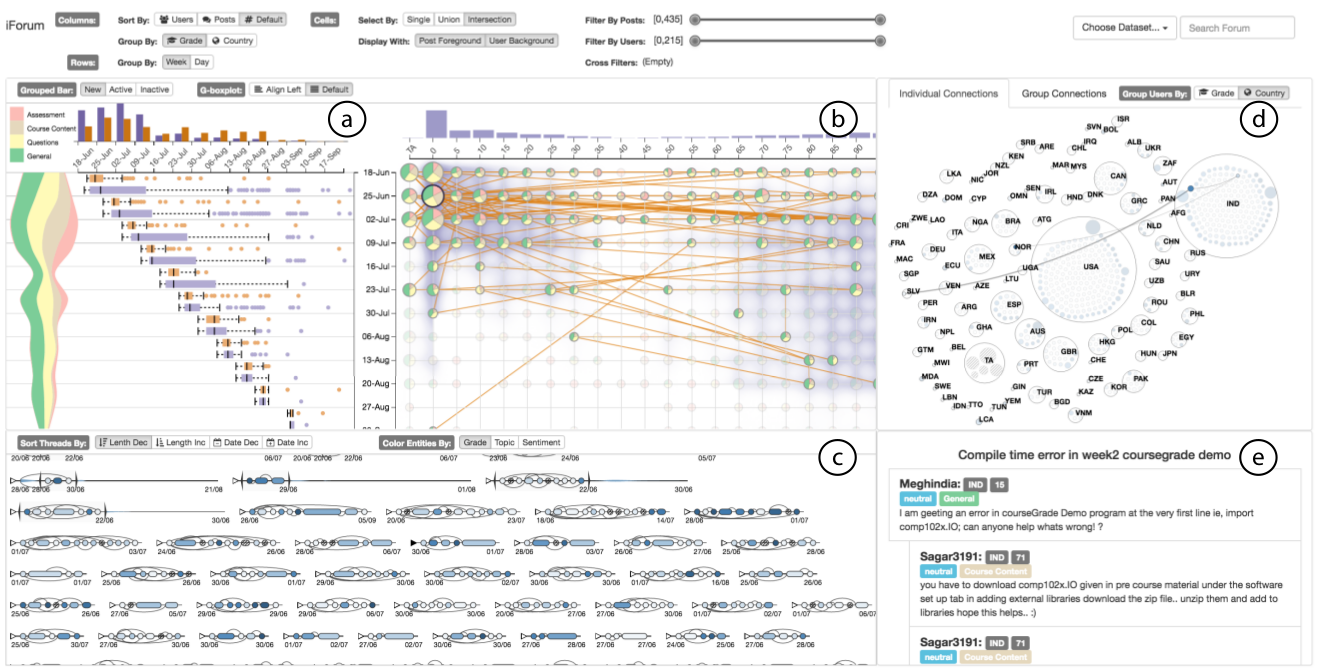
\includegraphics[width=.5\textwidth]{images/fu.png}
\end{figure}


\subsection{Analyzing collective actions}
Studies that consider collaboration usualy try to identify the intentions by studying the student's behavior and the message publications.


\paragraph{Detecting collective action}  In a 250 strong \gls{col}, \cite{Rehm2015} compare on-task users, those showing engagement and high performance, with off-task users.  They use questionnaires to relate the different behaviors to the users' hierarchical position in the \gls{col} social network.  They found a positive correlation not invalidating their hypothesis of an influence of the actor's social network position onto his learning. % With \gls{sna} tools this results can tested in larger online networks.

\cite{Wang2016} are other researchers interested in the learning~of off-topic and on-topic users.  After a detailed analysis of forum messages, they demonstrate that on-topic users, that is high-order thinking users displaying constructive and interactive behaviors in the forums, have more learning gain than off-topic learners.  In conclusion, the authors advocate for an off-topic discussion detector mechanism to guide users back on more constructive grounds.

In \citep{Chua2017}, the authors' approach is to study the turn-taking among discussion posting.  They identify different types of conversation and the following for users: loner, replier, initiator without reply, initiator who respond, active social learner, active social without turn-taking, reluctant active social learners.  Beside their valuable categorization, an important result is that they observe more engagement from recurrent posters, that is poster reply to comment made to their initial posts.

If the importance of collective action for learning is agreed upon, the difficulty is identifying it at scale.  It is a complex process needing content, temporal and social network analysis.  The previous studies justify the importance of a detailed content analysis but they relied on human intervention limiting their potential to scale up.
% Only recently papers tried to tackle the problem automatically.

\paragraph{Scaling up}

\cite{Dascalu2017,Boroujeni2017} are the first big scale attempts that we found taking in account time, message content, social and dialogue structure.  Each model the students' dynamics with a mixture of \gls{nlp} techniques (bags of words, \gls{lda}, word dictionaries) and \gls{sna} (eg. block models) applied to big temporal datasets.  \cite{Dascalu2017}'s dataset contains  3,685 contributions from 179 participants and spans 2 years.  \cite{Boroujeni2017} use 2 datasets of respectively 7,699 and 12,283 messages written by 1,175 and 1,902 participants.

\cite{Dascalu2017} proxy collaboration with a Cohesion Network Analysis score applied to synchronous chat room discussions.  It correlates significantly with human discussions' analysis but is not tested to identify collective actions as the learners were forced by pedagogical design in collaborative groups.

\cite{Boroujeni2017} analyze the influence of the course structure (timing and amount of staffs' publications) on the forum structure, content and on the social network of learners.  They are able to show the independence of forum content and the social network structure over the course structure that was only linked to the forum structure (number of posts).  They also report that although some learners do not publish often, they still have an important impact in forums because they can trigger discussions on course topics.  Finally, the authors recommend combining forum activity prediction model with content analysis to support instructors focusing on important discussions.

These two studies exemplify the possibility to get collective actions indicators based on content, structure and time, and as in \citep{Ezen2015} push for better support tools for tutors.
% had previously successfully applied an unsupervised \gls{nlp} clustering technique for synchronous discussions to asynchronous one.  They conducted their experiment with final aggregated data and recognize that end users would need a real time support with a more detailed content analysis.  

\begin{figure}[b]
  \small{
    \caption{\label{fig:convis}
      Convis Dashboard \citep{Hoque2016} helps explore conversations.  On the left, the topics found in the forum using \gls{lda} and organized hierarchically.  In the middle, the colored rectangles show a sentiment analysis for each message. Each message is linked to his author place on a semi-circle and thus creating a network. Finally, on the right, Convis display the detail of the conversation.
  \centering
  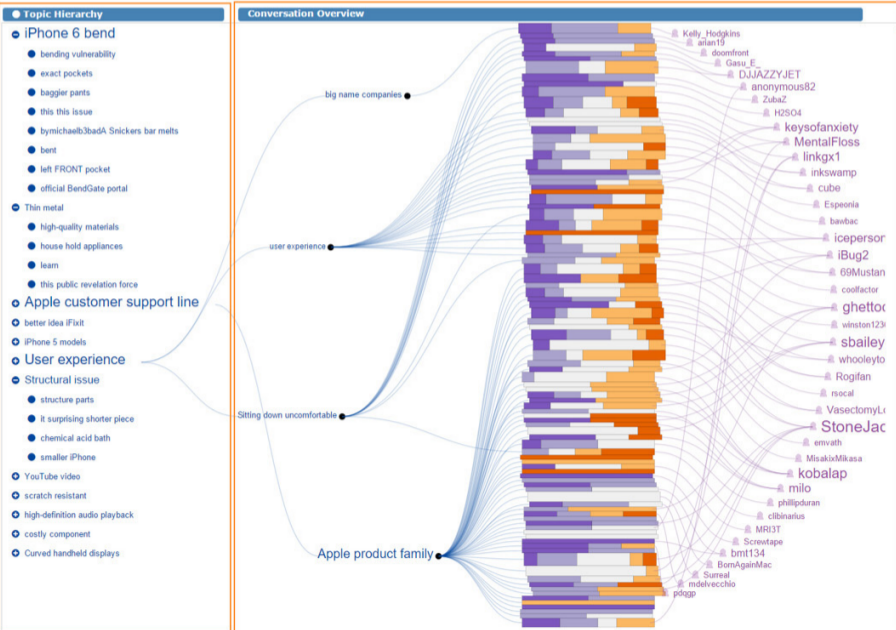
\includegraphics[width=.5\textwidth]{images/convis.png}
    }}
\end{figure}

\subsection{Visualizations as support tools}

Visualization as supporting tools have been used successfully in teaching contexts. \cite{Heer2012} classify the important visualization types and \cite{Emmons2017,Leeuwen2014} advocate their generalization to support all \gls{lms} users.

\paragraph{Exploration and awareness tools}
% on importance of visualization for group dynamics
\cite{Medina2016} use a \gls{ldb} to provide quick and precise feedback with his Behavioral Awareness Mechanism.  They tackle the problem of portability and provide dynamic feedback across several platforms to 24 students working on collaborative projects.  They use communication, coordination, motivation, performance and satisfaction indicators to operationalized collective actions.  Other studies showed how group awareness, rapid feedback about collective action, and visual narratives \citep{Yousuf2015} are beneficial to the students' engagement, even if no content analysis is done \citep{Davis2017,May2011,Medina2016}.
\cite{Davis2017} evaluated the impact a radar type visualization given to students in a two \glspl{mooc} and giving them awareness on what previous sessions learners had done at the same time of the course.  Their visualization had a positive impact only on older students.  It did improve significantly the younger students' activity in the forums.

Generally, as note \cite{Qu2015}, there is a  ``need to develop both advanced data mining methods to reveal patterns from MOOC data and visualization techniques to convey the analytical results to end users and allow them to freely explore the data by themselves''.
With VisForum, \cite{Fu2017}  answers to \cite{Qu2015}'s call.  VisForum  (Figure.~\ref{fig:fu}) provide a visual analytic system to interactively explore the forum of a \gls{lms}.  The complex interface helps the tutor group users and compare them to gain insights on the general forum dynamic in terms of structure but also sentiment analysis.
Convis from \cite{Hoque2016} is an explorative visualization that also satisfy \cite{Bull2016}'s recommendation for negotiable user models.   Convis (Figure.~\ref{fig:convis}) is a forum exploration tool designed around a topic model that evolves with users' feedback.   It facilitates finding insightful messages from discussions with hundred of them. 
Finally, \cite{Guo2017} propose TieVis, an original scalable visualization to track explore and analyze dynamics in interpersonal links, like those we could have between the actors mentioned in the previous section.

The limit of these researches is their complex visualizations.  iForum required an extensive explanation from the designers to help the instructor grasp what was shown.  Similarly, in Convis some users reported difficulty to use the visualization efficiently and in TieVis the authors recognized that some of their visualizations were not intuitive.

\begin{table*}[t]
  \begin{tabular}{lllrrllp{0.14\textwidth}}
    \toprule
    \multicolumn{1}{c}{\multirow{2}{*}{Dataset}} & \multicolumn{ 1}{p{0.07\textwidth}}{\multirow{2}{*}{Discussion}} & \multicolumn{ 1}{p{0.07\textwidth}}{\multirow{2}{*}{Message}} & \multicolumn{ 1}{p{0.07\textwidth}}{\multirow{2}{*}{Author}} & \multicolumn{2}{c}{Time} & \multicolumn{ 1}{c}{\multirow{2}{*}{Structure\sup{ii}}} & \multicolumn{ 1}{c}{\multirow{2}{*}{Extra\sup{iii}}} \\ [.1cm] \cline{ 5- 6}

    \multicolumn{ 1}{c}{source} & \multicolumn{1}{c}{(\#)} & \multicolumn{1}{c}{(\#)} & \multicolumn{1}{c}{(\#)} & \multicolumn{1}{p{0.08\textwidth}}{Span (days)} & \multicolumn{1}{c}{Precision\sup{i}} & \multicolumn{ 1}{l}{} & \multicolumn{ 1}{l}{} \\ \hline

    Coursera (2018) &  &  & \multicolumn{1}{l}{} & \multicolumn{1}{l}{} &  &  &  \\ [.2cm]
    HR & \multicolumn{1}{r}{499} & \multicolumn{1}{r}{1004} & 638 & 989 & ms & W, G \& S & V, C \& Sub. \\
    UFM & \multicolumn{1}{r}{1318} & \multicolumn{1}{r}{9460} & 4609 & 1022 & ms & W, G \& S & V, C \& Sub. \\ \hline
    Moodle (2009) &  &  & \multicolumn{1}{l}{} & \multicolumn{1}{l}{} &  &  &  \\ [.2cm]
    FFL & \multicolumn{1}{r}{348} & \multicolumn{1}{r}{1490} & 19 & 78 & s & T & Reading data, Att.~up/download, Citations. \\ \hline
    Hangouts (2018) &  &  & \multicolumn{1}{l}{} & \multicolumn{1}{l}{} &  &  &  \\ [.2cm]
    VUIC & \multicolumn{1}{r}{5} & 7297 & 96 & 327 & s & G \& S & - \\ \hline
    Coursera (2017) &  &  & \multicolumn{1}{l}{} & \multicolumn{1}{l}{} &  &  &  \\ [.2cm]
    PP & \multicolumn{1}{r}{868} & \multicolumn{1}{r}{2548} & 1112 & 365 & [1 h; 2 m] &W, G \& A & V \& C \\
    PML & \multicolumn{1}{r}{1135} & \multicolumn{1}{r}{4157} & 982 & 240 & [5 h; 1 m] & W, G \& A & V \& C \\
    VA & \multicolumn{1}{r}{248} & \multicolumn{1}{r}{549} & 311 & 728 & [1 d; 1 y] & W \& A & V \& C \\
    \bottomrule
  \end{tabular}
  \caption{\label{tab:datasets}List of datasets and courses that we use to experiment our \gls{ldb}.  \sup{i}When data was scrapped, the dates were in humanized format (eg. 6 month ago, 23 minutes ago), therefore the precision varies with posts' ages.  Recent posts can be compared with greater precision than older ones. We give the intervals in which the precision varies in hours (h), days(d), month (m) and year (y).  \sup{ii}The forum structure is given by the existence of different forum types: Weekly (W), General (G), Technical Support (S), Thematic (T) or Assignment (A) related.  \sup{iii}Extra information is often available, such as messages up votes (V), comments (C), subscription (Sub.) or attachment (Att.). }
\end{table*}

It is clear that visualizations can help creativity and holistic thinking; improve the ability to make effective inferences while translating or making visual analogies reinforces conceptual development; impact cognition, help sense-making and understanding \citep{Klerkx2014}.  \cite{Twissell2014} although in agreement with \cite{Klerkx2014} clarify the visualizations limits : 
\begin{inparaenum}[\itshape a\upshape)]
\item different learning styles, natural differences in learners have a significant impact on the way diagrams are perceived, visualized and understood
\item visualizations do not equally affect all types of learning activities.
\end{inparaenum}

\paragraph{Visualizations' effectiveness}

The study from \cite{Anaya2016} investigate how to reinforce student collective actions in the \gls{lms} dotLRN.  Noticeably they focus on directly helping the students, by designing a comprehensible tree-based visualization explaining to the student why they received a recommendation to act more collectively and how having a higher-order thinking behavior would be beneficial to them.
The engineer students working on a collaborative project reported to understand the tool and generally found it useful.

Nevertheless, precaution has to be taken with visualizations for young learners because in their research \cite{Lonn2015} found that a \gls{ldb} could have undesired side effects on teenagers.  Analyzing students in a summer camps remedial program, they reported that extensive usage of a \gls{ldb} shifted some mastery goal willing students to willing the lesser goal of competency proof.  The opposite was not witnessed.  Unfortunately, some students abandoned their initial motivation to only care about the grade or the \gls{ldb}'s feedback.

This last experiment justifies that although we aim to support tutors with explorable visualizations, we will consider topic based visualizations rather than user-based ones.  Topic-based visualizations do not emphases individual actions and, therefore, should damper the motivations to trick the system by adopting a superficial behavior.


\section{Explorable collective dynamics model}
\label{section:4}
In this section we detail our datasets and present the model we are going to use to analyze the collective dynamics from them.
% our firsts visualizations for exploring collective dynamics.

\subsection{Dataset collection}
Table~\ref{tab:datasets} Lists seven datasets collected between 2017 and 2018.  They are organized in four groups based the datasets' origins.
The datasets contain forum information from the following online courses:
\begin{itemize}
\item Coursera (2018), a database extraction for a Human Right (HR) and Understanding Financial Markets (UFM) courses.
\item Moodle (2009), a database extraction without message content for a French as Foreign Language (FFL) course.
\item Hangouts (2018), a JSON export from the VUIC's G Suite for Education.  It has the data from 5 chat rooms setup-up by university staff for the staffs or the students.
\item Coursera (2017), a saving of online courses using selenium webscrapper.  The dataset is then transformed and stored as a CSV file to be processed by a Python engine. It has messages' content but approximates the timestamp.  Three courses are available: Python Plotting (PP), Python Machine Learning (PML) and African Towns (AT) an urban planning course.
\end{itemize}

\subsection{The implicit relationship's strength}
\label{ssec:strength1}

\paragraph{Basic message relationship strength}
Figure~\ref{fig:discussion} gave a first example were the messages' closeness was translated in interaction's strength for actors.  In that example, the strength was either null, low or high.  In practice the strength $s$ could be anything in $[0;1]$.

We propose to define the relationship strength between two messages as a function of time, topics and actors.  This translates the idea that the message relationship depends on :
\begin{description}
\item[{Who}] wrote them.  Do the messages' authors have already interacted together before ?  Is the author a super poster, a lonely lurker ? One will probably consider a message differently depending on his relationship to the message's author.
\item[{Time}] Obviously the delay between two messages influence the strength of their relationship.  But keeping that fixed, the time of posting may also have an impact on the relationship's strength.  For example, the same messages posted by the same people may be linked differently, if the first message was posted at 11~pm and the second at 6~am or if the first was posted at 8~am and the second à 3~pm.  Although the influence of the publishing time delta will diminish as time intervals get bigger.  If you and your friend exchange letters every 6 months, it probably does not matter if that happens in July and January or in March and September.
\item[{Content}] should also play an import role in the way messages relate to one another.  The difficulty is to reliably automate content analysis, but \gls{nlp} techniques exist to push in that direction.
  
\end{description}
\begin{figure}[b]
  \centering
  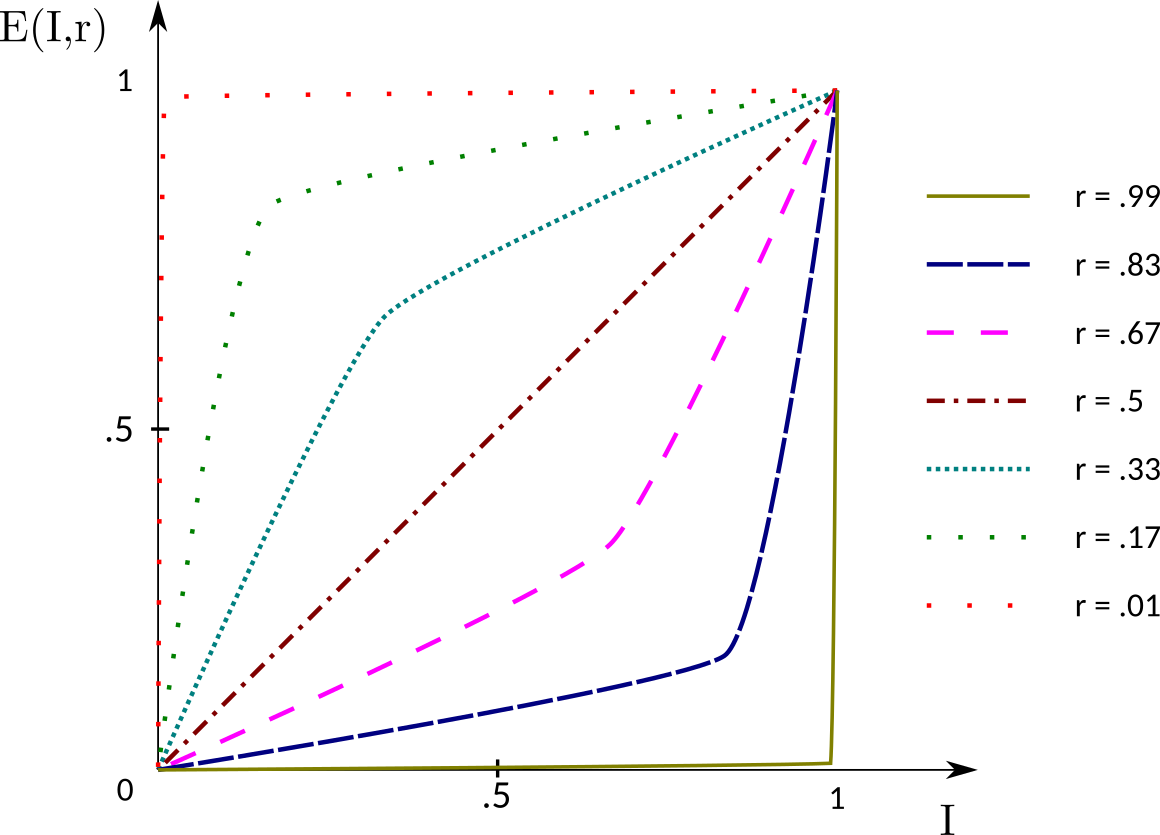
\includegraphics[width=.5\textwidth]{images/func.png}
  \small{
    \caption{\label{fig:func} Graphical proposition for the function  $I(s,r)$ of the messages' interaction strength. $s$ is the ``internal'' strength of two messages based on content, time and social network structure.  $r$ is ``external'' requirement, it is a parameter set by the observer.
    }}
\end{figure}

\paragraph{Required message correlation}

As we said earlier, deducting the causal relationship between messages is difficult because one has to guess what is the real intention of message's author.  To avoid making spurious deduction, we propose to make the relationship strength dependent on a parameter set interactively by the observer.  We call it the \emph{required message correlation} $r$ ($r\in[0;1]$).  If the observer set $r \approx 0$ then, for him, the requirement for a message to be linked to other messages is weak and interactions between messages, actors and topics will be common.  This would probably lead to  overly complex and unusable dynamics metrics and visualizations.  On the opposite if $r\approx 1$, the requirement is high, meaning that the observer wants linked messages to be close in time, have a lot of topic overlap and be written from closely connected author.  In that case messages, actor and topics will hardly have any relations with one another and no dynamic will be possible or visible.

\begin{figure}[t]
  \centering
  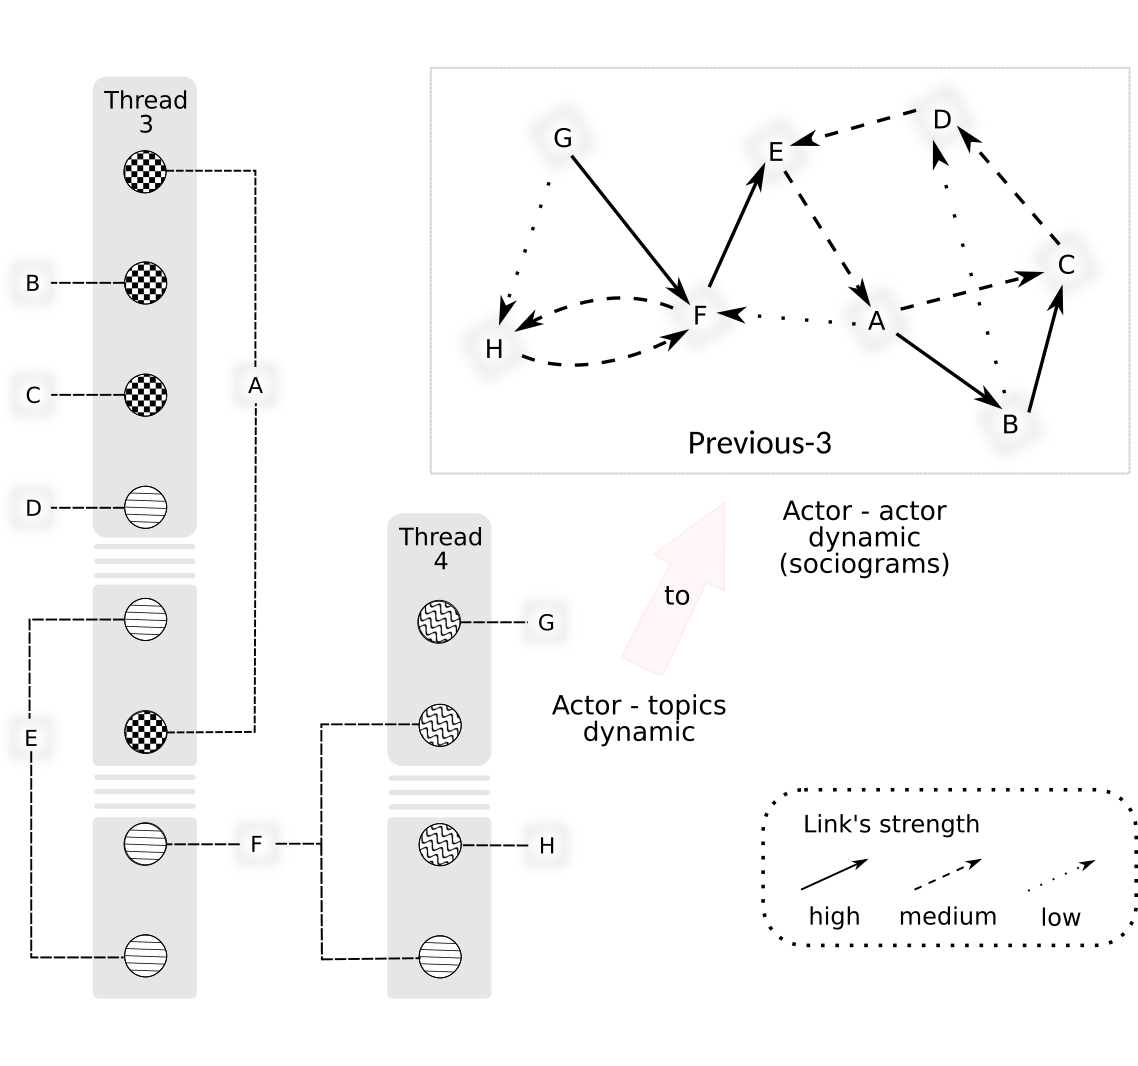
\includegraphics[width=.5\textwidth]{images/cycles.png}
  \small{
    \caption{\label{fig:cycles}
      Interactions cycles built from a bi-party actor-message graph  (Thread 1 and 2) transformed  to as an actor graph.  Dotted arrows denotes weaker links.
    }}
\end{figure}
 

\subsection{Collective dynamic model}

\paragraph{Causal interaction strength}
We define the causal interaction's strength $I$ between two messages as the measure of interaction taking in account the intention of exchange.  It is a function of $s$ and $r$, where $s$ is the ``internal'' message correlation, independent of the intention, based on topic, time and actor closeness, and $r$ is the required message correlation. $r$ observer's evaluation of intended interactions between the messages.  $I$ should satisfy:
\begin{align*}
  \forall \quad s' \in ]0;1[, \quad \left \{
  \begin{aligned}
    &\lim\limits_{r \to 0} I(s',r) = 1 \\
    &\lim\limits_{r \to 1} I(s',r) = 0
      \end{aligned}  \right .
\end{align*}
and its graph should look like Figure~\ref{fig:func}.  For any $s'$ if $r\approx 1$ (requirement high), $I$ should be stay low.

We care about this relationship because it's based on $I$ that we build the actor and topic dynamics.  In Figure~\ref{fig:cycles}, we give a more complete example than Figure~\ref{fig:discussion}.  Not only Actor $D$ will connect to $C$ but he will also connect to $B$ and potentially to $A$, as his message is part the Thread 3 started by $A$.
There is several way we could connect authors of same thread messages.  In Figure~\ref{fig:cycles} we limited ourselves to the previous 3.  That is beyond three ``ancestors'' we consider the correlation between the messages to be null ($s=0$).  Hence, if $D$ had published on the same topic as $A$, $B$ and $C$ he would have been connected to $A$, but since he was not so strongly connected to $C$, $s$ drops to $0$ before the interaction could reach $A$.  For the illustration purpose, each time we go back one time step or change topic, the message correlation drops from high to medium, medium to low or disappear.  Other ways of connecting the messages could have been in a ``star'' formation, that is connecting all user the the Thread initiator, or only to the previous 1, or to all the previous users.

The results of this manipulation is a temporal actor--actor network and a temporal topic-topic network that can be represented by a weighted oriented graph.  Snapshots of that network for the PP dataset is presented in Figure~\ref{fig:evolution}

\paragraph{Identifying collective actions}

Once we have the actor-actor and topic-topic networks from $s$,  we want to identify potential collective actions based on the networks' structures.

We make the hypothesis that the most collective actions are among actors part of a cycle.  By cycle we mean a thread with a recurrent author, for example (Figure~\ref{fig:cycles}): $$A \to B \to C  \dashrightarrow D  \dashrightarrow  E  \dashrightarrow A$$.

This pattern is visible in the Thread 3 and denotes that a user, here $A$, posted two non consecutive messages in the same thread.  And since $C$ is acting collectively with $A$ and $A$ with $F$, $C$ is also interacting in some way with $F$, and $H$, but not $G$.  If we follow the direction of arrows, there is no cycle including $G$.  In fact $G$ published an message and disappeared.  We have no evidence that the answers he got had an impact on him.  That is why the first condition to have a collective action, is recurrent interactions.  \cite{Chua2017} found them important too.


\section{Firsts visualizations}
\label{section:5}

\begin{figure}[b]
  \small{
    \caption{\label{fig:pipeline} Data Analysis cycle. Regular updates or extraction from the \gls{lms} feed data repositories used processed to a unified model.  Then \gls{sna} and \gls{nlp} techniques are used to generate the actor-actor and topic-topic networks dynamics.  The visual engine use that pre process data to generate interactive visualizations served to the \gls{lms} interface via common APIs.  Finally the observe can interact wit the visualizations and explore the topic-topic dynamics.
    }}
  \centering
  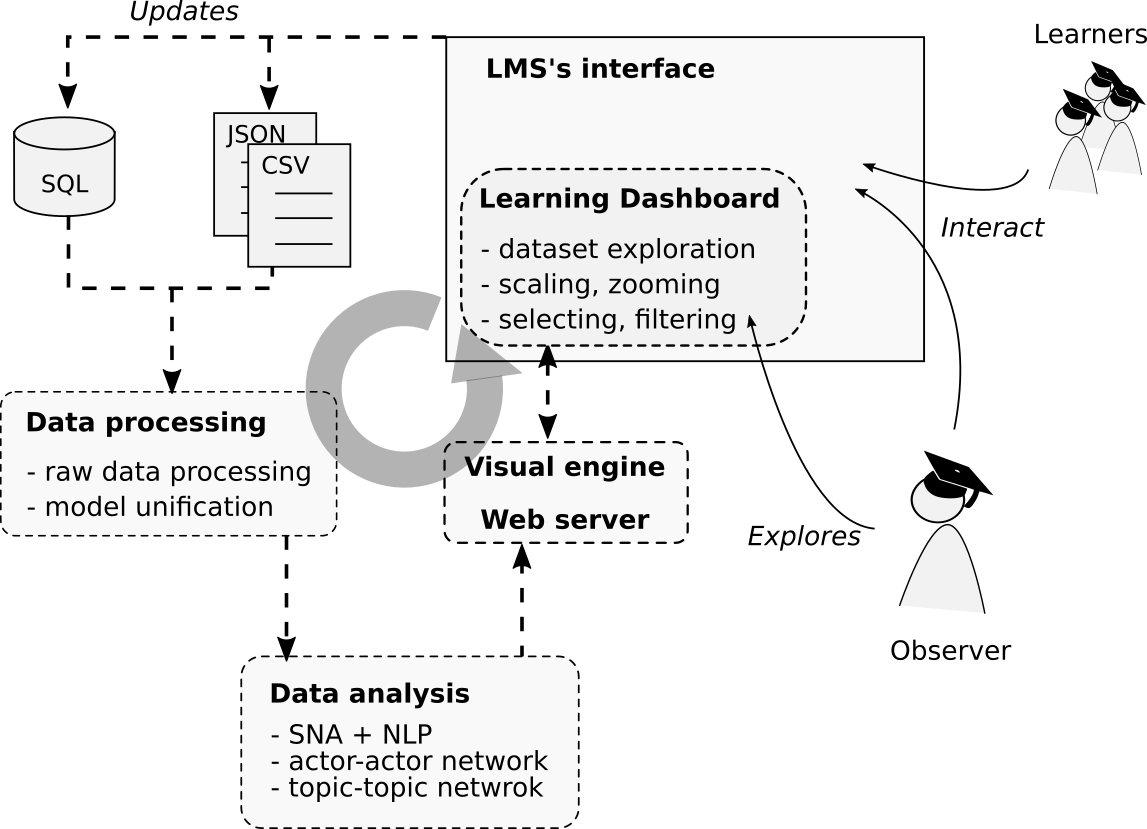
\includegraphics[width=.5\textwidth]{images/pipeline.png}
\end{figure}



We present three visualizations from our work in progress.  They were made separately each testing an element of the global conception model (Figure~\ref{fig:pipeline}).

The visualization from the hangout data tests the interaction, dataset exploration scaling needs.  The work with Moodle concerns data pre processing and standalone web server integration with common \gls{lms}.  The Coursera dataset is used to test \gls{nlp} and \gls{sna} techniques to uncover the collective activity indicators.

\begin{figure*}[t]
  \centering
  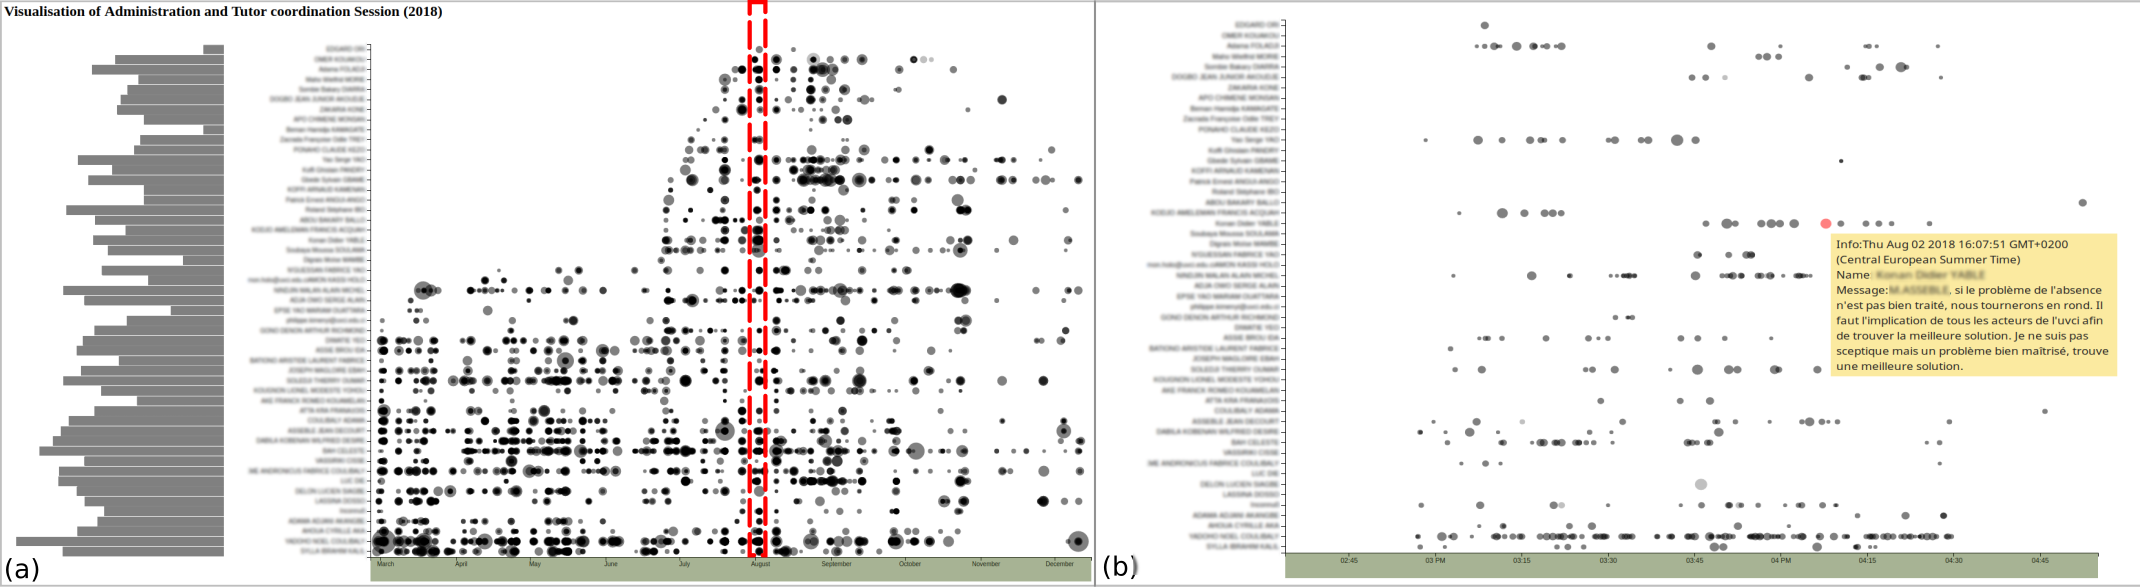
\includegraphics[width=\textwidth]{images/uvci_paysage_flou}
  \small{
    \caption{\label{fig:hgconv}
      Detail of VUIC conversation taking place in 2 hours.  Each circle is a message, and hovering over them brings up its content.  The circle's size is proportional to their content's length.  Message are layered vertically by actors.  On the left is an indication of the actors total messages count.
    }}
\end{figure*}

\subsection{Hangout dataset}

\paragraph{Tutor's survey}

We conducted a survey in July 2018 and ask the tutors their need for the collective dynamics visualization.  here is what came out of the results.
From the results, we understand that the collective dynamics will be noticeable by looking at the messages. and the forum chat.


\paragraph{First explorable \gls{ldb}}

The hangout dataset is slightly different from the other datasets in that it comes from 5 chat rooms.  Therefore it does note contains as much structure as the other dataset.
We used it to test the interaction and exploration interface.  Starting from a JSON file, it has been entirely processed in javascript but in the future, we plan to pre process in python as we did for the previous dataset.

In Figure~\ref{fig:hgconv} we show the main learning Dashboard on the left.  At the extreme left is a histogram of message count for each user.  Users are represented vertically in the middle with their names, and then comes along the time axis the messages plotted as circles proportional to the message's length.  We see here data from tutor reunions spanning from March 2018 to December 2018.
In the right pane, we made a zoom on the 2 hours period framed in red.  We the mouse hovers a message, its contents pops-up.  The interaction function, panning, zooming, mouse hovering provide the user a minimal exploration toolkit for this dataset.


\begin{figure*}[t]
  \centering
  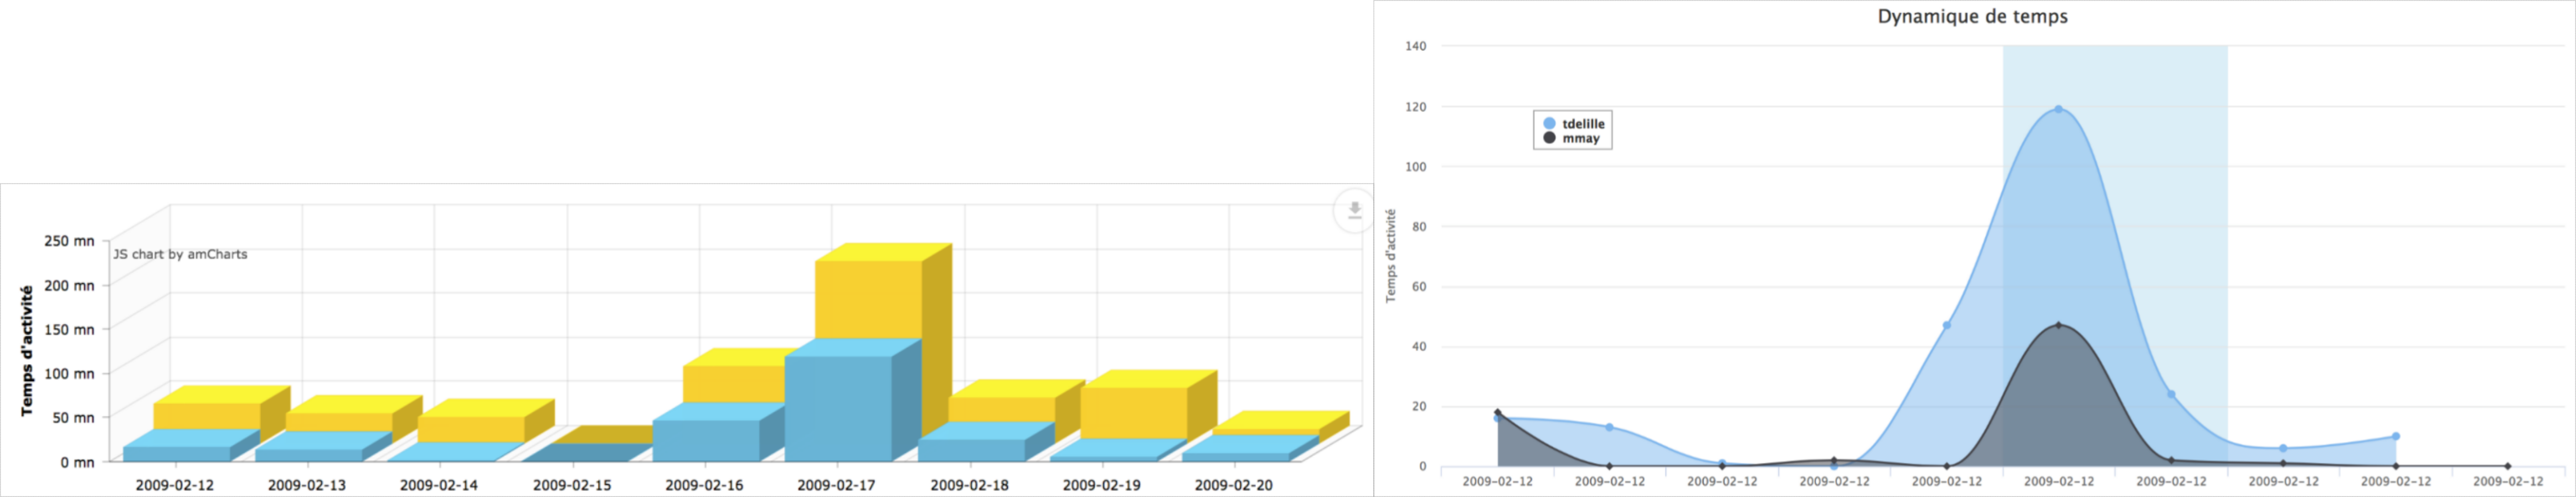
\includegraphics[width=\textwidth]{images/dynco.png}
  \small{
    \caption{\label{fig:dynco}
      Visualizations from the FFL dataset.  On the left, a comparison of an actor on-task and off-task activity obtained by tracking the presence or absence of significant interaction with the interface.  On the right, is the comparison of two users activity along the time axis.
    }}
\end{figure*}


\subsection{Moodle dataset}
The Moodle dataset contains information about the authors' messages, messages timestamp, messages' views, and actors' activities on the \gls{lms}, file attachment up and downloads.  We use the information about the activity types to identify active time from idle times.
On top of the dataset, we built a web application with an interactive interface enabling to choose a user and see visualizations corresponding to his activity. Figure~\ref{fig:dynco} shows visualizations examples obtain from that dataset.  On the left visualizations, in yellow,  we plotted for the selected user the total time spent on the \gls{lms} day per day.  It is possible to change the time range used for plotting in order to better scale the visualization.  On the same visualization, in blue, we  plotted the active time for the same user.
On the right visualization, we compared the activity time of two users.  We see that although the display similar activity patterns along the time axes, one is generally more active than the other.

\subsection{Coursera's dataset}
We have two Coursera datasets.  We used the one from 2017 to start to implement our collective activity indicator.  The second dataset, from 2018, will be used in following design iterations as it was collected to recently to be exploitable.

\begin{figure*}[t]
  \centering
  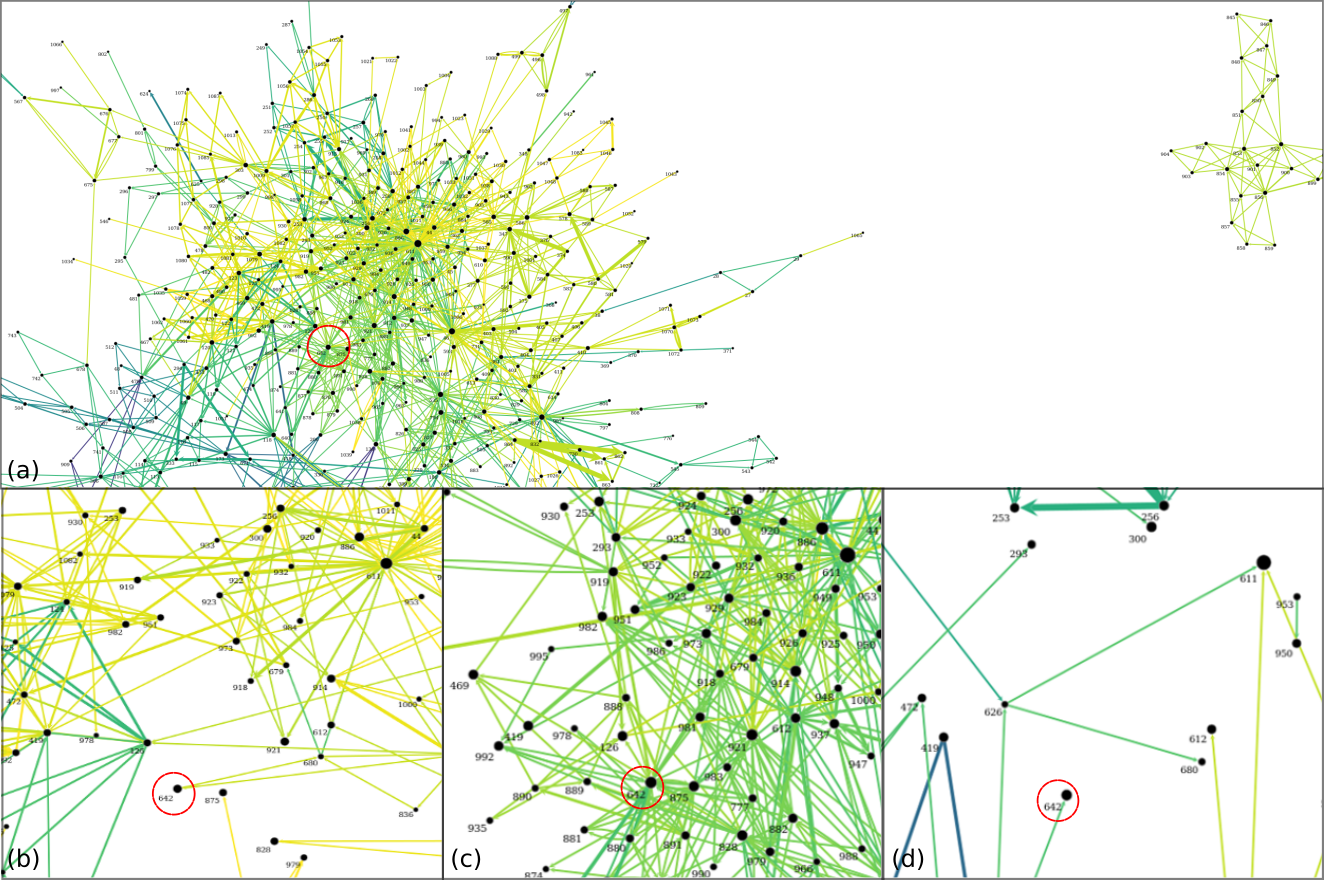
\includegraphics[width=\textwidth]{images/evolution.png}
  \small{
    \caption{\label{fig:evolution}
      At the top (a) is half of compound yearly actor-actor network built from the PP dataset (see Table \ref{tab:datasets}).  Nodes are users.  They are linked based on their proximity to the previous three actors who published in the same discussion.  Colors show different discussions.  The three bottom images (a), (b) and (c) are closeup around actor 578 during the \nth{2}, \nth{3} and \nth{4} quarters of the year.  We can see how the network changes around him.  The arrows' width depends on the actors' closeness in discussions, the actors' relations' occurrences and the number of votes that the answer got.
    }}
\end{figure*}

Figure~\ref{fig:evolution} tries to illustrate the actor--actor dynamics.  This is an intermediate visualization that is used for analysis purposes and will not be presented to the end users for two reasons:
\begin{inparaenum}[\itshape a\upshape)]
\item it give superficial information for someone that does not access to raw data,
\item it represents the actors as nodes and as we noted in section~\ref{section:3} we would rather have visualizations showing topics or depersonalized dimensions.
\end{inparaenum}
We present it here to illustrate what a social network looks like and zoomed and reduced to the three quarters snapshots (b), (c) and (d) it become a bit more comprehensible.
% In (a) user posts a message and gets a reply from user 579.
                                                    %                                                     and facilitate the visualization of what we build our collective indicator around, actor-network cycles.

\section{Perspectives and Conclusion}
\label{section:6}

\subsection{Perspectives}
\paragraph{Limits} Although we have started to test our model scalability and portability with different datasets, we do not yet have the results and we could find that cycles in actor--actor or topic--topic networks are not significant to measure collective action.
Also, our \gls{ldb}'s portability rests on the assumption that will be able to extract periodically, every few minutes, hours or days, data from the main \gls{lms}.  This will not hold for all \glspl{lms}.  Furthermore, we hope to integrate our \gls{ldb} back in the main \gls{lms} using APIs.  That will require proper authorizations.

Concerning the visualizations' development, we need to implement on the same dataset the \gls{sna} started with the PP dataset (Figure~\ref{fig:evolution}), \gls{nlp} analysis and extend the exploration's functions experimented with the Hangout dataset (Figure~\ref{fig:hgconv}).

\paragraph{Perspectives} Once our prototype fulfills all stages of the pipeline (Figure~\ref{fig:pipeline}), for the datasets we already have, our next step will be to test it with tutors from VUIC.   48 of them already participated in a survey in July 2018.  27 were not satisfied or unsure about their current tools' effectiveness to monitor their students' work.   At the same time, 39 agreed or strongly agreed that ICTs could help their students collaborate and 40 that collaboration was important for learning.
In the experiment with VUIC, we will certainly run into difficulties to process the VUIC content dataset because Ivorian french is not standard french and we will not be able to use, as is, common \gls{nlp} tools such as grammar parsers from Python's Nltk library.  But we hope to get promising feedback from the tutors about the usefulness of our prototype to monitor the collective actions of their students.

\subsection{Conclusion}
In this paper, we presented a model to detect collective activities from the forums' discussions.  We based our model on an internal message distance and an external parameter set by an observer.  Doing so, the collective dynamics that we measure is adaptable to the observer context and knowledge.  We avoid creating causal relationships between the messages, facilitating the portability of our approach to courses covering different domain and having significantly different populations.  For example, we suppose that an observer would only have to set his time requirement higher to observe interesting collective dynamics in a short course and set it lower if the course took several months.

Our model is the continuation of recent works in the field of data analysis and data visualization.  \gls{la} is at a turning point where a lot of attention is moving to support tools rather than fully automated learning solutions \citep{Kone2018,Baker2016}. We hope that this model will help tutors and, further, students discover the topic--topic dynamics in their \glspl{mooc} and support collectives activities so beneficial to learning.

\vfill 

\bibliographystyle{apalike}

\small{\bibliography{bib-csedu19}}

\vfill
\end{document}
